% Hier kommen zunaechst generelle Einstellungen fuer LaTeX:
\documentclass[11pt,titlepage]{article}     % Allgemeine Einstellungen fuer LaTeX:
                                            %  - Format des Textes: article
                                            %  - Schriftgroesse   : 11
                                            %  - Titelseite

\usepackage{german}                         % Sorgt dafuer, dass das Papierformat A4 verwendet wird, die
                                            % deutschen Umlaute zur Verfuegung stehen, feststehende
                                            % Bezeichnungen wie Inhaltsverzeichnis, Zusammenfassung auch in
                                             % deutscher Sprache erscheinen, usw.

\usepackage[T1]{fontenc}
\usepackage{epsf}  
\usepackage{epsfig}                          
%\usepackage{isolatin1}                      % Umlaute koennen direkt ueber die Tastatur eingegeben werden
\usepackage{float}

\setlength{\parindent}{0mm}                 % Keine Einrueckung am Absatzanfang
\setlength{\parskip}{3mm}                   % Leerraum zwischen den Zeilen
\setlength{\headheight}{5mm}               % Hoehe der Kopfzeile

\usepackage{textcomp}                       %f"ur �C und �
\usepackage{a4wide}                        % kleinere Seitenr"ander als bei article

%%%%%%%%%%%%%%%%%%%%%%%%%%%%%%%%%%%%%%%%%%%%%%%%%%%

%Br�che
 %  \begin{equation}
  %   f(x,y) = \frac{\sin x \cos y}{dx dy}
  % \end{equation}

%Mit dem folgendem Befehl kann man einen Seitenumbruch erzwingen:
\pagebreak

%Darstellung ohne Gleichungsnummer

%\begin{displaymath}
%\end{displaymath}

%{Einbinden von Bildern}

%\begin{figure}[h]
 % \begin{center}
 %   \epsffile{frogduck.eps}
 % \end{center}
 % \caption{Der Frosch und die Ente}
 % \label{frosch}
%\end{figure}

% Auf Abb. \ref{frosch} kann man sich mit \verb| \ref{frosch} | beziehen.

% Einbinden des Kapitels Schlusswort.
%\include{schlusswort}

% ein paar Befehle fuer Latex:

% \boldsymbol: fett und schraeg
% \bf x: x fett
% \cdot: Skalarprodukt-Punkt
% \dot{}: Punkt ueber Buchstabe
% \label{}: Name fuer Gleichung oder Abbildung um Verweise machen zu koennen
% \ref{}: Verweis auf Gleichung oder Abbildung
% \frac{]{}: Bruchstrich
%   Darstellung Matrix oder Vektor (Anzahl c ist Anzahl der Spalten):
% \begin{array}{c c c}
%   2 & 1 & 0 \\
%   1 & 2 & 0 \\
%   0 & 0 & 0
%   \end{array}
% $ ... $  : Um im Text mathematische Schreibweise darzustellen mit $ einrahmen
% \int_{}^{} : Integral
% x_{} : Index unten
% x^{} : Index oben
% \noindent verhindert Zeileneinschub nach einer Gleichung oder Abbildung
% \left[ und \right] stellt grosse eckige Klammern dar, geht auch mit allen anderen Klammern
% bei geschweifter Klammer aber ein bissel anders: \left\{ und \right\}
% \tilde{} : schlange ueber Buchstabe
% \partial : partielle ableitung
% \, : kleiner Abstand
% ~ : auch kleiner Abstand und die Zeichen werden nicht durch Zeilenumbruch getrennt


%%%%%%%%%%%%%%%%%%%%%%%%%%%%%%%%%%%%%%%%%%%%%%

% Festlegen des Inhaltes der Titelseite

\author{Simon~Kamaryt, Max~Schmidt, Jan~..., Sinan~Teske }
\title{Chancen heutiger Energiekonzepte im Jahr 2030\\ WS 06/07\\ (Grundlagen wissenschaftliches Arbeiten) }

% Hier beginnt das eigentliche Dokument:
\begin{document}

% Erstellt das Titelblatt
\maketitle

\thispagestyle{empty}                       % Auch auf dieser Seite keine Kopfzeilen
\tableofcontents                            % Erstellt das Inhaltsverzeichnis
\newpage                                    % Seitenwechsel

% Ab dieser Seite gibt es Kopfzeilen mit Seitenzahl und Kapitelueberschrift
\pagestyle{headings}

% Der Seitenzaehler wird auf 1 gesetzt
\setcounter{page}{1}

% Und jetzt kommt der eigentliche Text. Kapitelueberschriften werden dabei (das gilt fuer das Format article)
% mit den Befehlen \section, \subsection und \subsubsection erzeugt.

\section{Aufgabenstellung}

\section{Formulierung der Kriterien}

\section{Prozessauswahl}

	\subsection{Wandlung von Wellenenergie}
	
		\subsubsection{technische Realisation}

Die Nutzung von Wasser f�r Energieumwandlungsanlagen besitzt seit jeher einen hohen Stellenwert in der menschlichen Geschichte. Bereits 1200 v. Chr. wurden die ersten Wassersch"opfr"ader erfunden\cite{wiki} und zur Wandlung von kinetischer Str"omungsenergie in mechanische Energie genutzt. Dies erm"oglichte u.a. die Anhebung von Wasser auf ein h�heres Potential sowie eine Bew"asserung der Felder mit deutlicher Ersparnis an Muskelkraft. Heute wandeln Pumpspeicherwerke bei "ortlich gro\ss en H�hendifferenzen die potenzielle Energie des angesammelten Wassers aus einem vorgelagerten Stausee in elektrische Energie um. Dabei wird die potenzielle Energie des Wassers durch den H"ohenunterschied in kinetische Energie gewandelt und anschlie\ss end in einer Turbine entspannt. Obwohl das gr"o\ss te Kraftwerk der Welt ein Pumpspeicherkraftwerk in Paraguay ist, und den Strombedarf von ganz Paraguay sowie dreizig Prozent des brasilianischen Strombedarfs deckt\cite{bund}, ist die Nutzung von Str"omungen auf dem Festland stark limitiert. Die Gewinnung von elektrischer Energie in gro\ss er Menge bleibt auf wenige Standorte beschr�ngt, weswegen diese Art der Energiewandlung hier nicht betrachtet wird.\\
Unter Wandlung von Wellenenergie werden hier drei verschiedene Verfahren beurteilt. Dazu z�hlen die Nutzung eines Rampensystems oder einer Pneumatikkammer sowie die Energiewandlung durch Hydraulikzylinder.\\
Das Rampensystem nutzt das Prinzip eines Wellenkonzentrators. Dazu werden zwei v-f�rmig angeordnete Barrieren zur Mitte hin konzentriert. Die Wellen werden so verst�rkt und flie\ss en nach �berwinden der Rampe durch eine Turbine, welche durch Verbindung zu einem Generator die zugef�hrte Energie speichert. Das Wasser gelangt anschlie\ss end zur�ck ins Meer. Die Anlage kann flexibel eingesetzt werden, da sie ein schwimmendes Offshore-Kraftwerk ist. Die folgende Abbildung zeigt das Funktionsprinzip des Projekts $Wave~Dragon$. 

\begin{figure}[H]
\begin{center}
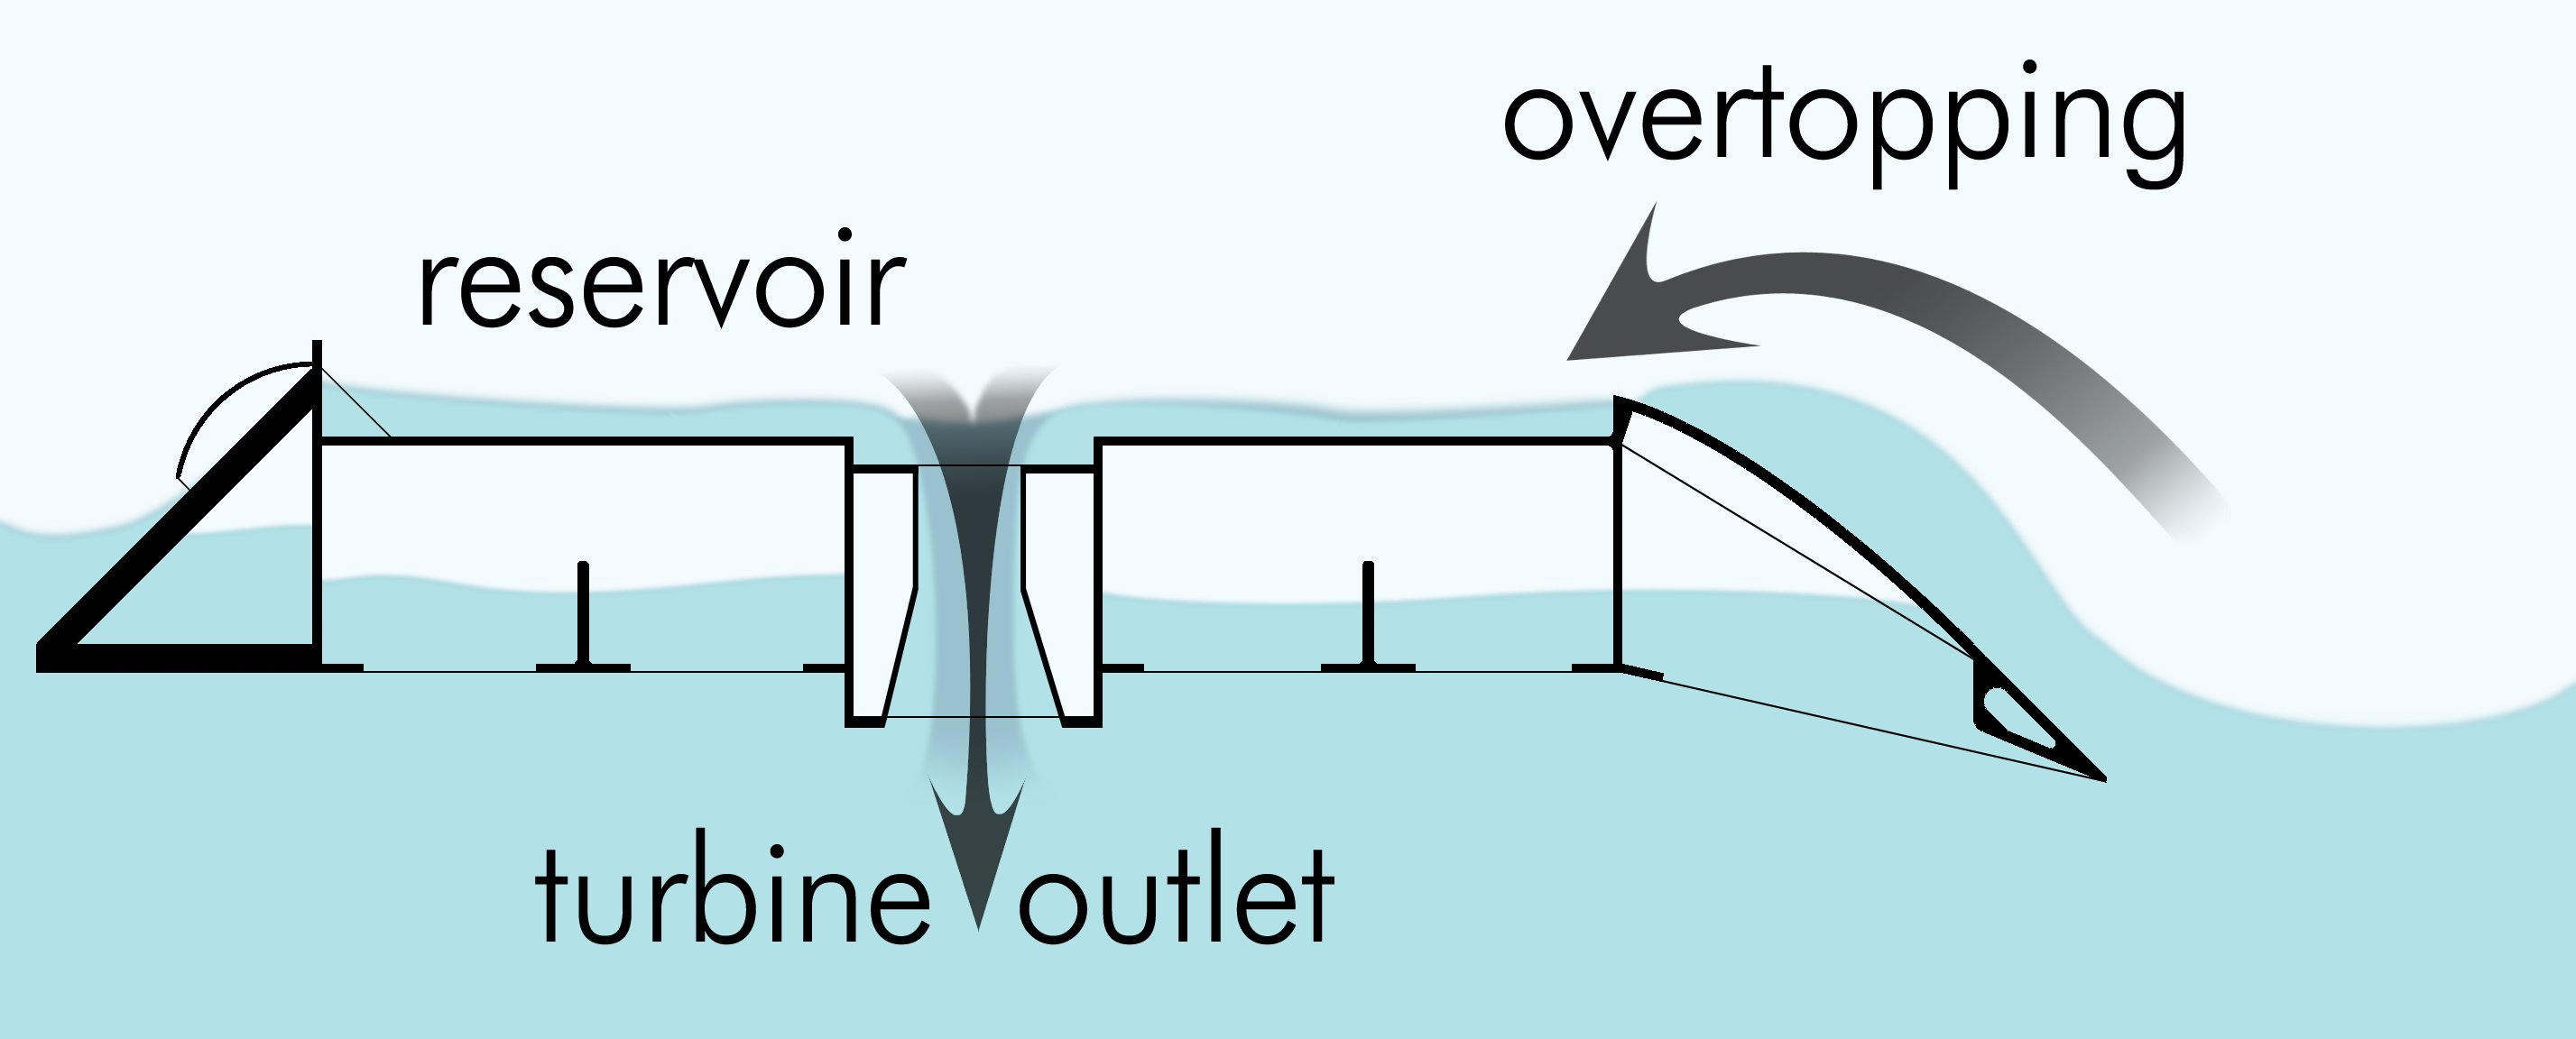
\includegraphics[width=9cm]{PrinzipRampe.jpg}
\caption{Prinzipskizze Wave Dragon\cite{wd}}
\end{center}
\end{figure}

Das weltweit erste Wellenkraftwerk funktioniert nach dem OWC-Prinzip ($oscillating~water~column$). Dazu wird jede Welle durch Betonr�hren in eine Pneumatikkammer geleitet, wobei weitere Betonr�hren auf einer anderen Seite in einer so genannten Wells-Turbine enden. Durch die Ein- und Ausleitung der Wellen zirkuliert die in der Kammer enthaltene Luft und treibt so eine Turbine an. Diese kennzeichnet sich durch ein symmetrisches Fl�gelprofil, welches senkrecht zum Luftstrom angeordnet ist, und ist somit unabh�ngig von der Str�mungsrichtung.

\begin{figure}[H]
\begin{center}
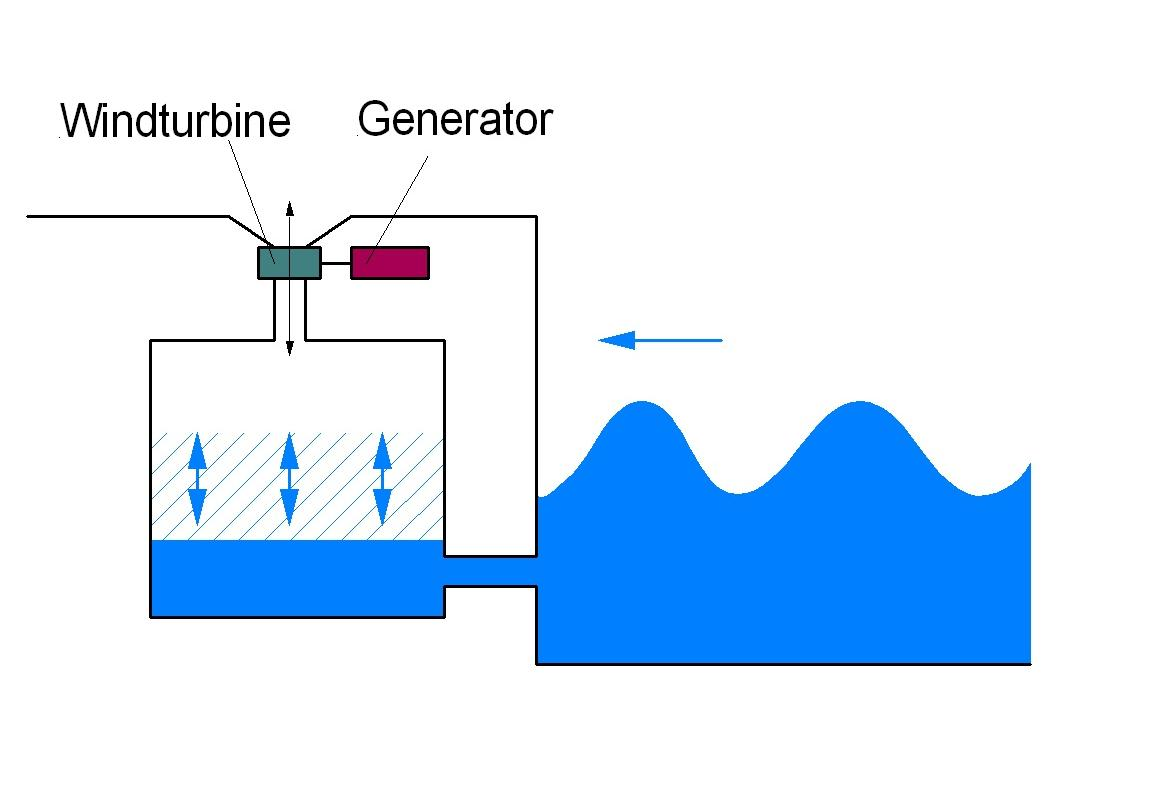
\includegraphics[width=9cm]{Kammer.jpg}
\caption{Prinzipskizze OWC\cite{wiki}}
\end{center}
\end{figure}

Eine weitere M�glichkeit zur Nutzung der Wellenenergie besteht in der Reihenschaltung von Modulen auf der Wasseroberfl�che, welche durch bewegliche Gelenke miteinander verbunden sind. In diesen Gelenken befinden sich Hydraulikzylinder, welche durch die Relativbewegung der der Module zueinander die enthaltene Hydraulikfl�ssigkeit in einen Ausgleichsbeh�lter leiten. Durch Zwischenschalten einer Turbine mit einem Generatoranschluss kann die Wellenenergie so gespeichert werden. Das System schwimmt etwa $50-60$ m �ber dem Meeresboden und wird durch drei Sicherheitsleinen befestigt\cite{pela}.

\begin{figure}[H]
\begin{center}
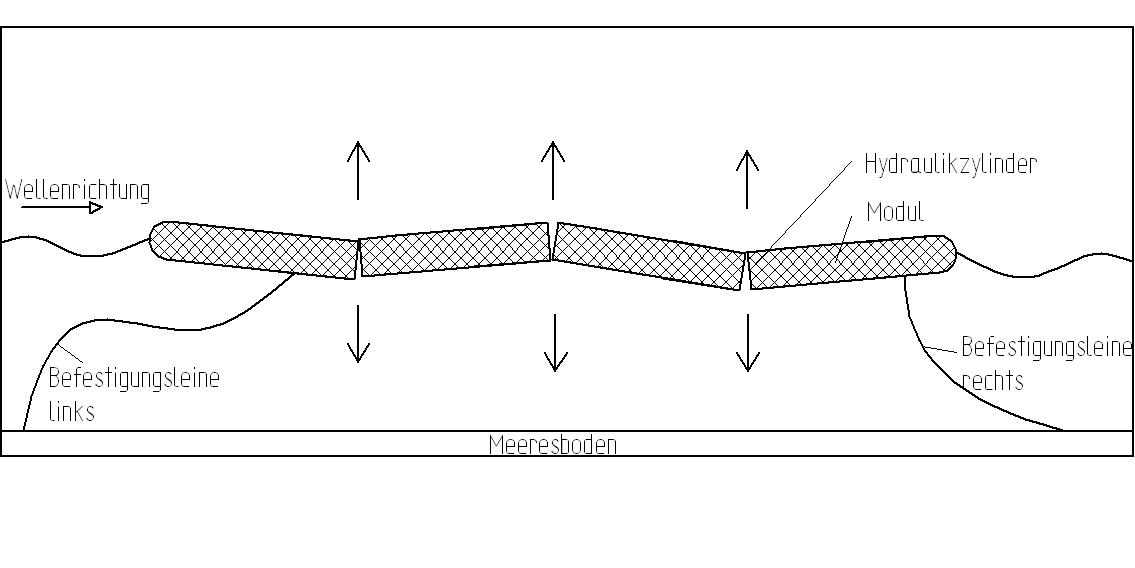
\includegraphics[width=11cm]{PrinzipPelamis.jpg}
\caption{Prinzipskizze Hydraulikzylinder}
\end{center}
\end{figure}

		\subsubsection{Bewertung}

	\subsection{Kernfusion}

	\subsection{k"unstliche Kohleerzeugung}

	\subsection{regenerative Energien}



\addcontentsline{toc}{section}{Literatur}

\begin{thebibliography}{99}
  \bibitem{wiki}					www.wikipedia.de\\
  													03.12.2006 
  \bibitem{bund} 							Dr.Daniel L�bbert, $Das~Meer~als~Eneriequelle$\\
  													Info-Brief der wissenschaftlichen Dienste des deutschen Bundestages
  \bibitem{wd}            www.wavedragon.net\\
                           07.12.2006
  \bibitem{pela}         www.oceanpd.com\\
                           03.12.2006
\end{thebibliography}

\end{document}